\documentclass[12pt]{article}
\usepackage{graphics}
\usepackage[top=1in,bottom=1in,left=1in,right=1in]{geometry}
\usepackage{alltt}
\usepackage{array}	
\usepackage{graphicx}
\usepackage{tabularx}
\usepackage{verbatim}
\usepackage{setspace}
\usepackage{listings}

\usepackage{amssymb,amsmath, amsthm}
\usepackage{zed-csp}
\usepackage[cc]{titlepic}

\usepackage{minted}
\usepackage[svgnames]{xcolor}


\title{SOEN 363: Data Systems for Software Engineers\\
\ \\
Assignment 1}
\author{Nathan Grenier}
\date{\today \\ Fall 2024}

\begin{document}
\begin{spacing}{1.5}
      \maketitle

      \newpage

      \begin{enumerate}

            \item[Q1.] [40 Points] Consider the following system description for a museum information systems:

                  A museum has multiple departments. A museum has collections. A collection belongs to a department.

                  Art-objects belong to a collection. An art-object has a unique acquisition number, object type, title, description, dimension, production date, and production
                  country. Examples of object types are paintings, sculptures, etc. An art-object may be linked to an artist. Some art-objects are just without one. An art-object belongs to a period (i.e. Roman Empire).

                  An exhibition takes place in a museum which exhibits various art objects from various collections. An exhibition has a start and end date, as well as a home department. Art objects may be borrowed temporarily from various museums for a specific exhibition.

                  \begin{enumerate}

                        \item[A)] [20 pts] Design a data model that implements the above description. Identify the entities, relations, attributes, keys, and their cardinalities. Identify strong and weak entities and relations, if applicable. Represent the end result in the form of an ERD diagram. single arrow - no arrow notation for cardinalities and single line - double line for partial and total participation [??].

                              \textbf{Note: The software I used couldn't do dashed underlined text. Therefore, bold + underline + italics represents a partial key.}

                              \begin{figure}[h!]
                                    \centering
                                    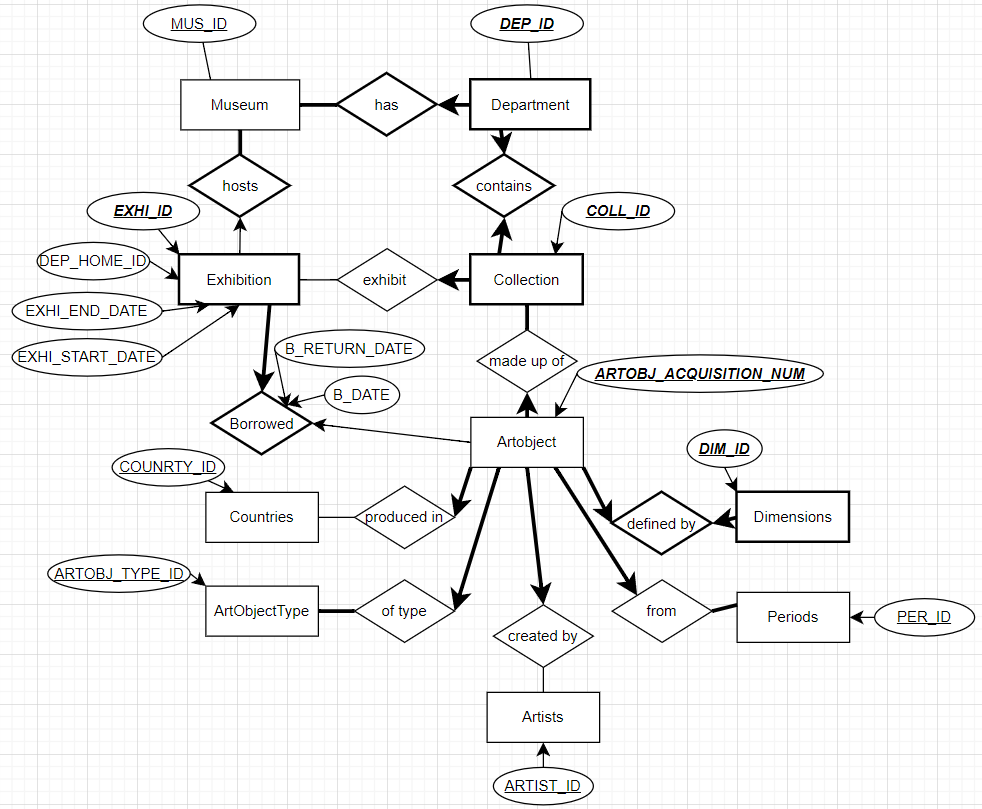
\includegraphics[width=1\textwidth]{q1/q1(chen).png}
                              \end{figure}

                              \newpage

                        \item[B)] [10 pts] Provide a DDL script for the above.

                              \inputminted[bgcolor=Beige, frame=lines, fontsize=\small, linenos, breaklines]{sql}{q1/db.sql}

                              \newpage

                        \item[C)] [10 pts] Provide a database instance that demonstrate an exhibition with local (from home department) and borrowed art objects.

                              \inputminted[bgcolor=Beige, frame=lines, fontsize=\small, linenos, breaklines]{sql}{q1/seed.sql}

                  \end{enumerate}

                  \newpage

            \item[Q2.] [40 Points] Consider the following system description to manage group or private lessons:

                  Consider an organization that offers group or private lessons (of various types, such as yoga, swimming, etc.) to clients. The organization owns or rents space (gyms, rooms, swimming pools) in various locations in possibly different cities across the province and each location is made available over some given schedule, where a schedule is essentially a sequence of day-time slots. E.g. “The EV-Building gym Room 7, in Montreal, is available for Judo classes on Sundays from 12 noon to 3PM, from September 1st to November 30th, 2024.” The length of a time slot is not fixed (and you are free to create schedules as you see fit). For example, a swimming lesson would normally be for half hour, but a Judo class would normally be for one hour.

                  A given location can only accommodate one lesson at any given time slot on a given day. The same type of lesson can be offered in both modes (private, group). For example, at the same location the organization would offer private swimming lessons and group swimming lessons.

                  The organization does not have permanent instructors, but it hires seasonal instructors of various specializations. An instructor would register with the system by entering their credentials (name and phone number) and specialization as well as to register their availability in one or possibly several cities. For example, “Grace (514 - ... ) is a swim instructor, available to work in Montreal and Laval."

                  Once registered, an instructor can subsequently take on possibly several offerings that the organization makes available. All offerings are made available to potential instructors, but only those that have been taken by instructors are made available to the public in order to attract clients. For example, “We offer private and group Judo classes in EV-Building on Sundays from 12PM to 3PM from 1.Sep to 30.Nov as follows: 12:00 - 13:00. Group. Instructor: ... 13:00 - 14:00. Group. ... 14:00 - 14:30. Private. ... 14:30 - 15:00. Private. ... We offer swimming classes at ... ... ”

                  \begin{enumerate}
                        \item[A)] [25 pts] Design a data model that captures the above description. Identify the entities, relations, attributes, keys, and their cardinalities. Identify strong and weak entities and relations, if applicable. Represent the end result in the form of an ERD diagram, using chen notation [??].

                              \begin{figure}[h!]
                                    \centering
                                    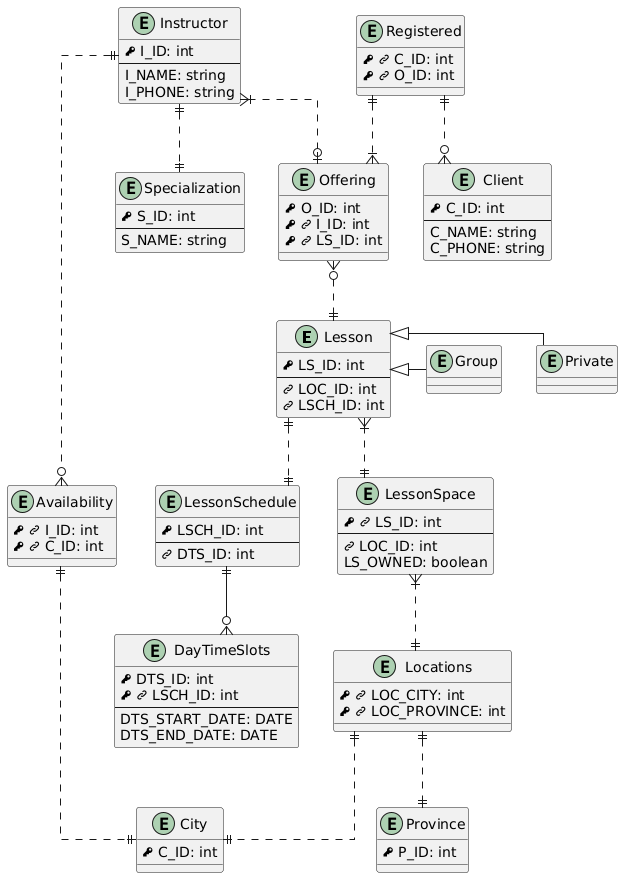
\includegraphics[width=0.9\textwidth]{diagrams/out/q2a(crow)/q2(crow).png}
                              \end{figure}

                              \newpage

                        \item[B)] [6 pts] Provide the schema and explicitly identify the domains of each attribute.

                              \inputminted[bgcolor=Beige, frame=lines, fontsize=\small, linenos, breaklines]{sql}{q2/db.sql}

                              \newpage

                        \item[C)] [9 pts] Provide a database instance that demonstrate offers to a sample instructor, one of which is accepted, one is rejected, and one is pending response. Demonstrate a group and a private lesson in your example.

                              \inputminted[bgcolor=Beige, frame=lines, fontsize=\small, linenos, breaklines]{sql}{q2/seed.sql}

                  \end{enumerate}

                  \newpage

            \item[Q3.] [20 Points] Represent the ERD of either questions in crow's foot notation using PlantUml [??], [??]. Make sure you submit both PlantUML source and the diagram image.

                  \textbf{Question 1 ERD (Crow's Foot Notation):}

                  \begin{figure}[h!]
                        \centering
                        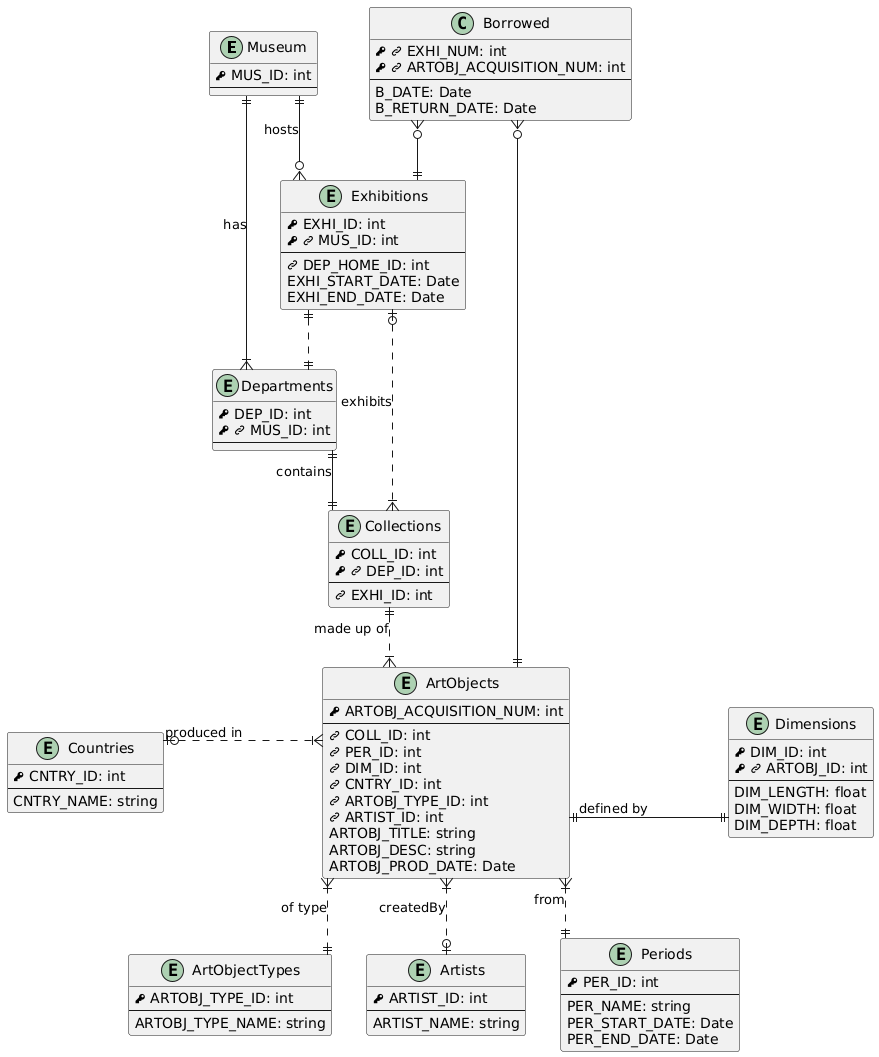
\includegraphics[width=1\textwidth]{diagrams/out/q1a(crow).png}
                  \end{figure}

      \end{enumerate}

\end{spacing}

\end{document}